\interlude{Knock-patterns\\[1.1em]\Large{}How to introduce real-world attacks by trying to prevent them}

\SetNextBackground{}
\begin{frame}{}
  \centering
  \includegraphics[height=\pageheight,page=1,clip,trim=0 30 0 60]{graphics/scientific/rosenpass-wireguard-attack-types}
\end{frame}

\SetNextBackground{}
\begin{frame}{}
  \centering
  \includegraphics[height=\pageheight,page=2,clip,trim=0 5 0 50]{graphics/scientific/rosenpass-wireguard-attack-types}
\end{frame}

\interlude{From merely knowing cryptography \\[0.6em] towards\\practicing cryptography}

\SetNextBackground{}
\begin{frame}{Real-World Impact---Working Definition}
  Something, that people rely on regularly and preceive as a trusted resource.
  \\[1.3em] Providing continuity.
\end{frame}

\SetNextBackground{}
\begin{frame}{Cryptography as an engineering process}
  \only<1,3>{
    \small
    \textbf{Maintained}
    \\ Provide bug fixes, updates, and improvements\only<1>{.}%
    \only<3>{---for the definitive resource on the security of the thing that you research.}
    \\[1.3em] \textbf{Suitable}
    \only<1>{\\ Efficient, available on the user's platform}%
    \only<3>{\\ Analyzing the security properties your target audience cares about.}
    \\[1.3em] \textbf{Usable}
    \only<1>{\\ High-quality documentation, user interface makes sense.}
    \only<3>{\\ Accessible and comprehensible to readers with vastly differing backgrounds and levels of expertise.}
  }
  \only<2>{
    \centering
    To apply this definition to a cryptography project,
    \\[1.3em] move away from one-time papers
    \\[1.3em] and towards providing the definitive resource on the security of your area of research.
  }
\end{frame}

\SetNextBackground{\includegraphics[width=\paperwidth,page=11]{hpke-in-avionics-slide-designs}}
\begin{frame}
  \begin{minipage}{.6\pagewidth}
    \centering
    Research is going to the moon.
    \\[3em]
    Engineering is going to the moon, routinely.
  \end{minipage}
\end{frame}

\SetNextBackground{}
\begin{frame}{Cryptography as a community process}
  \only<1>{
    \centering

    Maintained, suitable, and usable
    \\[1.3em] is more than a single person can achieve on their own.
  }
  \only<2>{
    \small
    \textbf{Dependable, persistent} (Maintained)
    \\ Provide bug fixes, updates, and improvements, event when you are indisposed.
    \\[0.6em] Maintain the resource as a team or community.
    \\[1.3em] \textbf{Client-centered} (Suitable)
    \\ Serving the client's needs, on their terms.
    \\[0.6em] Accept the client as an expert on their use-case.
    \\[1.3em] \textbf{Empowering} (Usable)
    \\ Grant a new super-power to the client.
    \\[0.6em] Turn, what previously was your special experise, into a mundane tool for the user.
  }
  \only<3>{
    \centering
    Empower client, team, (and critics).
    \\[1.3em]De-center your own expertise and status.
  }
\end{frame}

\begin{frame}{}
  \centering
  Real-world success is about getting people to use, be excited about, reccomend, and depend on your stuff.
  \\[1.3em] To make this happen, you need to be a project-diplomat
  \\who invests a lot of time to schmooze with the users.
\end{frame}

\SetNextBackground{\reflectbox{\includegraphics[width=\paperwidth,page=10]{hpke-in-avionics-slide-designs}}}
\begin{frame}{}
  \raggedleft
  \begin{minipage}[fullwidth]{.50\pagewidth}
    \centering
    To practice cryptography, you must:
    \\[1.3em] \textbf{Make a choice to depart from merely-knowing.}
    \\[1.3em] \textbf{Accept the loss of your singular status as an expert.}
    \vspace{1em}
    \hrule
    \vspace{1.3em}
    \textbf{Become a member of}
    \\[1.1em] \textbf{and serve}
    \\[1.1em] \textbf{the project community.}
  \end{minipage}
\end{frame}
